\documentclass[mathserif]{beamer}

% Clears navigation bar and symbols
\setbeamertemplate{footline}[page number]{}
\setbeamertemplate{navigation symbols}{}
\usetheme{Copenhagen}

\usepackage{amsmath}
\usepackage{amsthm}

\newtheorem{thm}{Theorem}
\newtheorem{prop}{Proposition}

\usepackage{tikz}
\usepackage{xcolor}

\tikzstyle{node} = [circle, node distance=0.5]
\tikzstyle{edgenode} =[rectangle, midway, fill=white, font=\color{black!50}\tiny]
\tikzstyle{line} = [draw, thick]
\tikzstyle{vec} = [draw, ->, -latex, ultra thick, orange]

\newcommand{\rplayer}{\textcolor{red}{Red }}
\newcommand{\bplayer}{\textcolor{blue}{Blue }}

\author{Gio Carlo Cielo Borje}
\institute{UC Irvine}
\title{Combinatorial Game Representation and Analysis of Snort}
\date{\today}

\setbeamercovered{transparent}
\begin{document}

\begin{frame}
	\maketitle
\end{frame}

\begin{frame}{Snort Description}
	\begin{description}
		\item [Two players] \rplayer and \bplayer
		\item [Board] map (usually planar)
		\item [Moves]
			\begin{itemize}
				\item \rplayer colors an available region red
				\item \bplayer colors an available region blue
			\end{itemize}
		\item [Constraints] no two regions can have the opposing color
		\item [Gameover] player with no moves loses
	\end{description}

	\vfill
	\pause
	\begin{figure}[h]
		\centering
		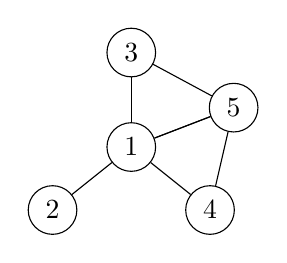
\begin{tikzpicture}
			\tikzset{every node/.style={circle, draw}}
\node (n1) at (2,1.8) {$1$};
\node (n2) at (1,1) {$2$};
\node (n3) at (2,3) {$3$};
\node (n4) at (3,1) {$4$};
\node (n5) at (3.3,2.3) {$5$};

\foreach \from/\to in {n1/n2,n1/n3,n1/n4,n1/n5,n1/n5,n3/n5,n4/n5}
{
	\draw (\from) -- (\to);
}

		\end{tikzpicture}
	\end{figure}
\end{frame}

\begin{frame}{Snort Demo: 1}
	\begin{figure}[h]
		\centering
		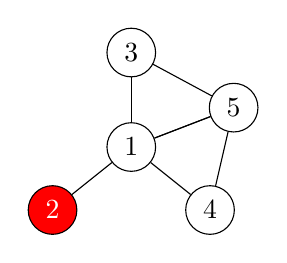
\begin{tikzpicture}
			\tikzset{every node/.style={circle, draw}}
\node (n1) at (2,1.8) {$1$};
\node[fill=red,text=white] (n2) at (1,1) {$2$};
\node (n3) at (2,3) {$3$};
\node (n4) at (3,1) {$4$};
\node (n5) at (3.3,2.3) {$5$};

\foreach \from/\to in {n1/n2,n1/n3,n1/n4,n1/n5,n1/n5,n3/n5,n4/n5}
{
	\draw (\from) -- (\to);
}

		\end{tikzpicture}
	\end{figure}
	\vfill
	\begin{center}
		\rplayer selects vertex $2$
	\end{center}
\end{frame}

\begin{frame}{Snort Demo: 2}
	\begin{figure}[h]
		\centering
		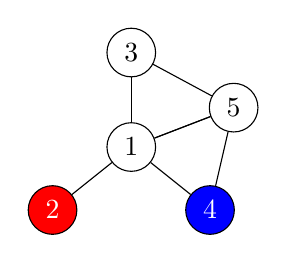
\begin{tikzpicture}
			\tikzset{every node/.style={circle, draw}}
\node (n1) at (2,1.8) {$1$};
\node[fill=red,text=white] (n2) at (1,1) {$2$};
\node (n3) at (2,3) {$3$};
\node[fill=blue,text=white] (n4) at (3,1) {$4$};
\node (n5) at (3.3,2.3) {$5$};

\foreach \from/\to in {n1/n2,n1/n3,n1/n4,n1/n5,n1/n5,n3/n5,n4/n5}
{
	\draw (\from) -- (\to);
}

		\end{tikzpicture}
	\end{figure}
	\vfill
	\begin{center}
		\bplayer selects vertex $4$
	\end{center}
\end{frame}

\begin{frame}{Snort Demo: 3}
	\begin{figure}[h]
		\centering
		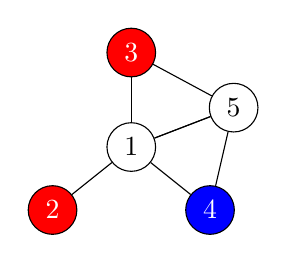
\begin{tikzpicture}
			\tikzset{every node/.style={circle, draw}}
\node (n1) at (2,1.8) {$1$};
\node[fill=red,text=white] (n2) at (1,1) {$2$};
\node[fill=red,text=white] (n3) at (2,3) {$3$};
\node[fill=blue,text=white] (n4) at (3,1) {$4$};
\node (n5) at (3.3,2.3) {$5$};

\foreach \from/\to in {n1/n2,n1/n3,n1/n4,n1/n5,n1/n5,n3/n5,n4/n5}
{
	\draw (\from) -- (\to);
}

		\end{tikzpicture}
	\end{figure}
	\vfill
	\begin{center}
		\rplayer selected vertex $3$
	\end{center}
	\begin{center}
		\rplayer player wins
	\end{center}
\end{frame}

\begin{frame}{Snort Classification}
	\begin{enumerate}
		\item Determinate
		\item Zero-sum
		\item Asymmetric
		\item Perfect information
		\item Sequential
		\item Normal-play
		\item Unfair
	\end{enumerate}
\end{frame}

\begin{frame}{Unfairness}
	\begin{thm}
		Snort is an unfair game.
	\end{thm}
	\pause
	\vfill
	\begin{proof}
		Any game that is a zero-sum, partisan, progressively-bounded game with
		no ties, has a winning strategy for a player that depends on the
		currently given state.
	\end{proof}
	\pause
\end{frame}

\begin{frame}{Snort: Progressively Bounded}
	\begin{lemma}
		Snort is progressively bounded.
	\end{lemma}
	\begin{proof}
		Given that there are n vertices and there are four
		vertex states, there is at most $o(4^n)$ possible
		game configurations. Hence, the state space is
		finite.

		Further, each move locks a particular vertex to a
		configuration which reduces the state space size.
		Consequently, there will be at most $O(n)$ moves
		before a gameover state is reachd.
	\end{proof}
\end{frame}

\begin{frame}{Unfairness}
	Conclusion:
	\begin{thm}
		Snort is an unfair game.
	\end{thm}
\end{frame}

\begin{frame}{Trivial Graph Families: Star Graphs}
	\begin{center}
		All star graphs are \textbf{N}-positions.
	\end{center}
	\vfill
	\begin{figure}[h]
		\centering
		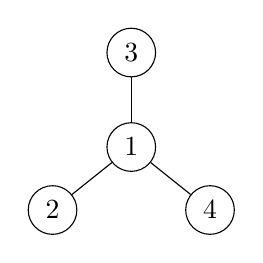
\begin{tikzpicture}
			\tikzset{every node/.style={circle, draw}}
\node (n1) at (2,1.8) {$1$};
\node (n2) at (1,1) {$2$};
\node (n3) at (2,3) {$3$};
\node (n4) at (3,1) {$4$};

\foreach \from/\to in {n1/n2,n1/n3,n1/n4}
{
	\draw (\from) -- (\to);
}

		\end{tikzpicture}
	\end{figure}
\end{frame}

\begin{frame}{Nontrivial Graph Families: Path Graphs}
	\begin{center}
		All path graphs are \textbf{N}-positions.
	\end{center}
	\vfill
	\begin{figure}[h]
		\centering
		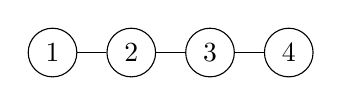
\begin{tikzpicture}
			\tikzset{every node/.style={circle, draw}}
\node (n1) at (1,1) {$1$};
\node (n2) at (2,1) {$2$};
\node (n3) at (3,1) {$3$};
\node (n4) at (4,1) {$4$};

\foreach \from/\to in {n1/n2,n2/n3,n3/n4}
{
	\draw (\from) -- (\to);
}

		\end{tikzpicture}
	\end{figure}
\end{frame}

\begin{frame}{Nontrivial Graph Families: Even Cycle Graphs}
	\begin{center}
		All even cycle graphs are \textbf{P}-positions.
	\end{center}
	\vfill
	\begin{figure}[h]
		\centering
		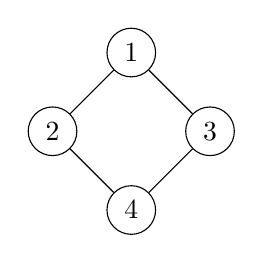
\begin{tikzpicture}
			\tikzset{every node/.style={circle, draw}}
\node (n1) at (2,2) {$1$};
\node (n2) at (1,1) {$2$};
\node (n3) at (3,1) {$3$};
\node (n4) at (2,0) {$4$};

\foreach \from/\to in {n1/n2,n1/n3,n2/n4,n3/n4}
{
	\draw (\from) -- (\to);
}

		\end{tikzpicture}
	\end{figure}
\end{frame}

\begin{frame}{Nontrivial Graph Families: Odd Cycle Graphs}
	\begin{center}
		All odd graphs are \textbf{N}-positions.
	\end{center}
	\vfill
	\begin{figure}[h]
		\centering
		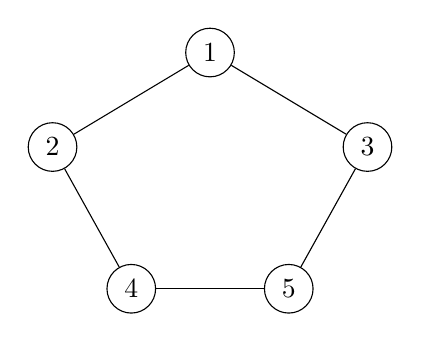
\begin{tikzpicture}
			\tikzset{every node/.style={circle, draw}}
\node (n1) at (3,3) {$1$};
\node (n2) at (1,1.8) {$2$};
\node (n3) at (5,1.8) {$3$};
\node (n4) at (2,0) {$4$};
\node (n5) at (4,0) {$5$};

\foreach \from/\to in {n1/n2,n1/n3,n2/n4,n3/n5,n4/n5}
{
	\draw (\from) -- (\to);
}

		\end{tikzpicture}
	\end{figure}
\end{frame}

\begin{frame}{Game Variants}
	Consider games of three players or more:
	\begin{itemize}
		\item The state space increases exponentially
		\pause
		\item Collusion is an important factor
		\pause
		\item Star graphs are still trivial
	\end{itemize}

	\pause
	\vfill
	Consider expanding the space between player pieces:
	\begin{itemize}
		\item Fewer valid board configurations
		\item Upperbound on state space is still the same
		\pause
		\item Star graphs are still trivial
	\end{itemize}
\end{frame}

\begin{frame}
	\begin{center}
		Thank you. Snort simulator and solver are available on GitHub: https://github.com/Hydrotoast/SnortSolver 
	\end{center}
\end{frame}

\end{document}
